\documentclass{standalone}
\usepackage{graphicx}	
\usepackage{amssymb, amsmath}
\usepackage{color}

\usepackage{tikz}
\usetikzlibrary{intersections, backgrounds, math}
\usepackage{pgfmath}

\definecolor{light}{RGB}{220, 188, 188}
\definecolor{mid}{RGB}{185, 124, 124}
\definecolor{dark}{RGB}{143, 39, 39}
\definecolor{highlight}{RGB}{180, 31, 180}
\definecolor{light_teal}{RGB}{107, 142, 142}
\definecolor{mid_teal}{RGB}{72, 117, 117}
\definecolor{dark_teal}{RGB}{29, 79, 79}
\definecolor{gray10}{gray}{0.1}
\definecolor{gray20}{gray}{0.2}
\definecolor{gray30}{gray}{0.3}
\definecolor{gray40}{gray}{0.4}
\definecolor{gray60}{gray}{0.6}
\definecolor{gray70}{gray}{0.7}
\definecolor{gray80}{gray}{0.8}
\definecolor{gray90}{gray}{0.9}
\definecolor{gray95}{gray}{0.95}


\begin{document}

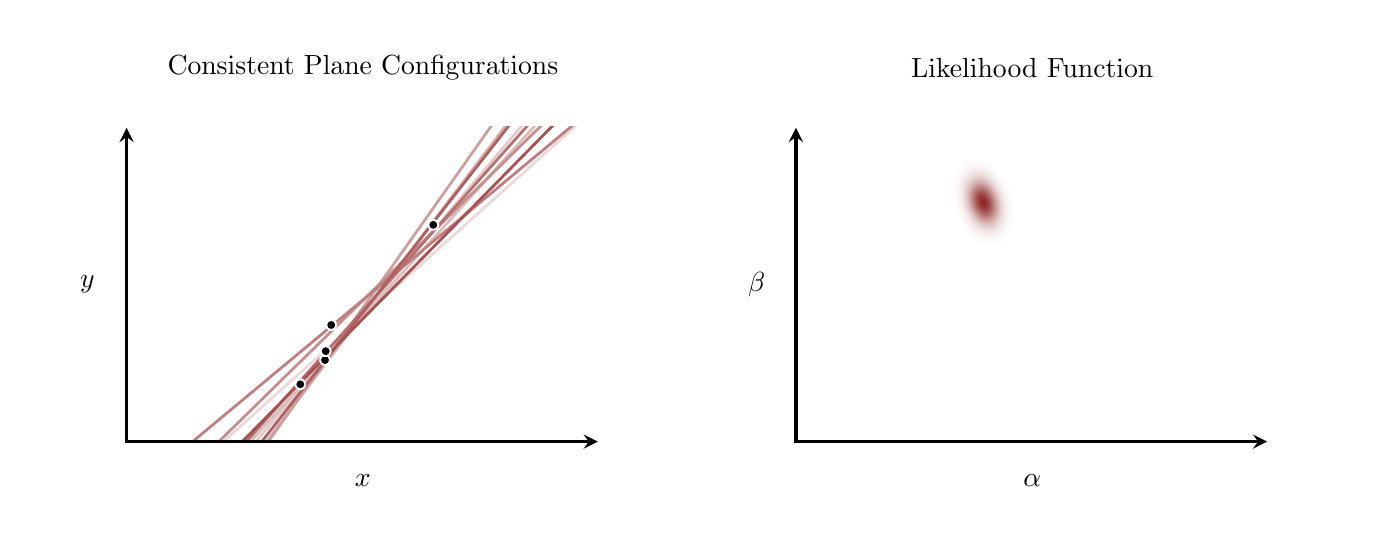
\begin{tikzpicture}[scale=1.0]

  \begin{scope}[shift={(0, 0)}]
    \draw[white] (-4.25, -3) rectangle (4.25, 3.25);  

    \node at (0, 2.75) { Consistent Plane Configurations };

    \begin{scope}
      \clip (-3, -2) rectangle (3, 2);
      
      \foreach \a/\b [count=\n] in {-0.413/0.896, -0.385/1.188, -0.415/1.111, -0.384/1.320, -0.300/1.416, -0.207/0.980, -0.201/0.832, -0.337/1.124, -0.359/1.278, -0.441/1.018} {
        \pgfmathsetmacro{\prop}{10 + 7 * \n};
        \colorlet{custom}{dark!\prop!white};
        \draw[domain={-3:3}, smooth, samples=30, line width=1, variable=\x, color=custom] 
          plot ({\x},{\a + \b * \x});
      }
    
      \foreach \x/\y in {-0.481/-0.964, -0.795/-1.272, -0.402/-0.519, -0.472/-0.851, 0.894/0.753} {
        \fill[white] (\x, \y) circle(0.075);
        \fill[black] (\x, \y) circle(0.05);
      }
    
    \end{scope}

    \draw [->, >=stealth, line width=1.25] (-3.00, -2.015) -- +(0, 4);
    \draw [->, >=stealth, line width=1.25] (-3.015, -2.00) -- +(6, 0);
    
    \node at (-3.5, 0) { $y$ };
    \node at (0, -2.5) { $x$ };
  \end{scope}
  
  \begin{scope}[shift={(8.5, 0)}]
    \draw[white] (-4.25, -3) rectangle (4.25, 3.25);  

    \node at (0, 2.75) { Likelihood Function };

    \begin{scope}
      \clip (-3, -2) rectangle (3, 2);
    
          \foreach \x [count=\n] in {1} {
        \pgfmathsetmacro{\prop}{10 + 7 * \n};
        \colorlet{custom}{dark!\prop!white};
        
      \foreach \i in {3, 2.95, ..., 0} {
        \pgfmathsetmacro{\prop}{100 * exp(-0.5 * \i * \i)};
        \colorlet{custom}{dark!\prop!white};
        \pgfmathsetmacro{\dy}{\i}
        \fill[custom, rotate={45 * 0.3926265}] (-0.2743352, 1.179362) circle (\i * 0.1215653 and \i * 0.1900241);
      }
    }
    
    \end{scope}

    \draw [->, >=stealth, line width=1.25] (-3.00, -2.015) -- +(0, 4);
    \draw [->, >=stealth, line width=1.25] (-3.015, -2.00) -- +(6, 0);
    
    \node at (-3.5, 0) { $\beta$ };
    \node at (0, -2.5) { $\alpha$ };
  \end{scope}
  
\end{tikzpicture}

\end{document}  